\documentclass[10pt]{beamer}

\usepackage[utf8]{inputenc}

\usetheme[progressbar=frametitle]{metropolis}
%\usetheme{ITS}
\usepackage{appendixnumberbeamer}
\usepackage{tikz}
\usepackage{tikzpeople}
\usetikzlibrary{shapes,fit}
\usepackage{xcolor}

\usepackage[operators,sets]{cryptocode}

\setbeameroption{hide notes} % Only slides
%\setbeameroption{show only notes} % Only notes
%\setbeameroption{show notes on second screen=right} % Both

\usepackage{amsmath}

\usepackage{adjustbox}

\usepackage{booktabs}
\usepackage[scale=2]{ccicons}

\usepackage{environ}

\usepackage{listings}

\usepackage{pgfplots}
\usepgfplotslibrary{dateplot}

%rectangles around nodes
\usetikzlibrary{calc}

%right of=30mm of X
\usetikzlibrary{positioning}

\usepackage{xspace}
\newcommand{\themename}{\textbf{\textsc{metropolis}}\xspace}

\usepackage{hyperref}


\title{Secure Steganography on ML-Based Channels}
\date{11. November 2022}
\author{Jeremy Boy}
\institute{Universität zu Lübeck}
% \titlegraphic{\hfill\includegraphics[height=1.5cm]{logo.pdf}}

\newsavebox\myboxa
\newsavebox\myboxb
\newlength\myhta
\newlength\mydpa
\newlength\myhtb
\newlength\mydpb
\newlength\maxht

\newcommand\CCCcolumns[3]{%
\begin{lrbox}{\myboxa}
  \begin{minipage}{0.3\linewidth}
  #1
  \end{minipage}%
\end{lrbox}%
\begin{lrbox}{\myboxb}
  \begin{minipage}{0.3\linewidth}
  #3
  \end{minipage}%
\end{lrbox}% 
\settoheight\myhta{\usebox\myboxa}%
\settodepth\mydpa{\usebox\myboxa}%
\addtolength\myhta{\mydpa}%
\settoheight\myhtb{\usebox\myboxb}%
\settodepth\mydpb{\usebox\myboxb}%
\addtolength\myhtb{\mydpb}%
\setlength\maxht{\myhta}%
\ifdim\myhtb>\myhta
  \setlength\maxht{\myhtb}%
\fi
\begin{minipage}[t][\maxht][c]{0.45\linewidth}
  #1
\end{minipage}\hfill
\begin{minipage}[t][\maxht][c]{0.1\linewidth}
  #2
\end{minipage}\hfill
\begin{minipage}[t][\maxht][c]{0.45\linewidth}
  #3
\end{minipage}%
}

\AtBeginSection{\frame{\sectionpage}}
%\AtBeginSection{}
%\AtBeginSubsection{\frame{\subsectionpage}}

\newcommand\blfootnote[1]{%
  \begingroup
  \renewcommand\thefootnote{}\footnote{#1}%
  \addtocounter{footnote}{-1}%
  \endgroup
}

\makeatletter
\newsavebox{\measure@tikzpicture}
\NewEnviron{scaletikzpicturetowidth}[1]{%
  \def\tikz@width{#1}%
  \def\tikzscale{1}\begin{lrbox}{\measure@tikzpicture}%
  \BODY
  \end{lrbox}%
  \pgfmathparse{#1/\wd\measure@tikzpicture}%
  \edef\tikzscale{\pgfmathresult}%
  \BODY
}
\makeatother


\newcommand\Vtextvisiblespace[1][.3em]{%
  \mbox{\kern.06em\vrule height.3ex}%
  \vbox{\hrule width#1}%
  \hbox{\vrule height.3ex}}

\begin{document}

\maketitle

\begin{frame}{Contents}
  \setbeamertemplate{section in toc}[sections numbered]
  \tableofcontents[hideallsubsections]
\end{frame}

\section{Secure Steganography and the Meteor Stegosystem}

\begin{frame}{Secure Steganography and the Meteor Stegosystem}
\centering
\begin{adjustbox}{max totalsize={.9\textwidth}{.7\textheight},center}
	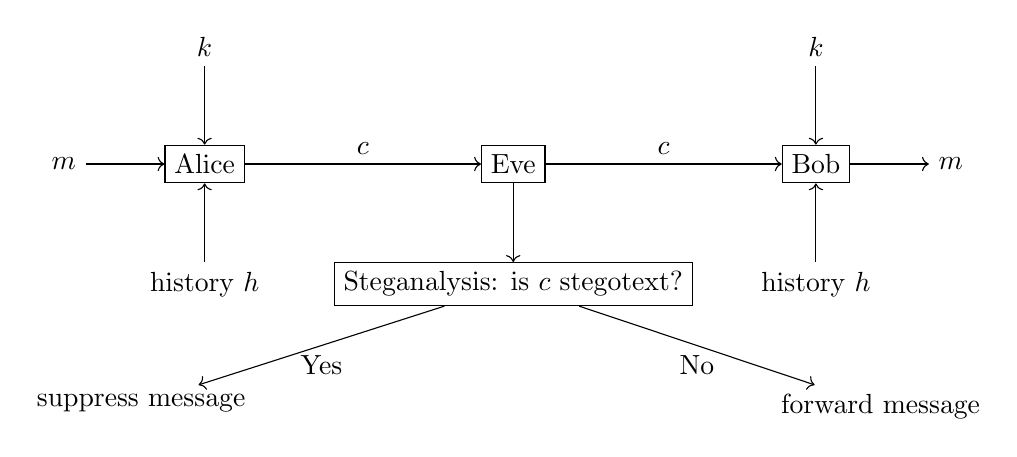
\begin{tikzpicture}
	  \node[rectangle, draw=black] (alice) {Alice};
	  \node[rectangle, draw=black, right=3cm of alice] (warden) {Eve};
	  \node[rectangle, draw=black, right=3cm of warden] (bob) {Bob};
	  \node[left=of alice] (m) {$m$};
	  \node[above=of alice] (k) {$k$};
	  \node[below=of alice] (h) {history $h$};
	  \node[right=of bob] (mb) {$m$};
	  \node[above=of bob] (kb) {$k$};
	  \node[below=of bob] (hb) {history $h$};
	  \node[rectangle, draw=black, below=of warden] (steganalysis) {Steganalysis: is $c$ stegotext?};
	  \node[below left=of steganalysis] (isstego) {suppress message};
	  \node[below right=of steganalysis] (notstego) {forward message};
	  \draw[->] (alice) -- node[above] {$c$} (warden);
	  \draw[->] (warden) -- node[above] {$c$} (bob);
	  \draw[->] (m) -- (alice);
	  \draw[->] (k) -- (alice);
	  \draw[->] (h) -- (alice);
	  \draw[->] (bob) -- (mb);
	  \draw[->] (kb) -- (bob);
	  \draw[->] (hb) -- (bob);
	  \draw[->] (warden) -- (steganalysis);
	  \draw[->] (steganalysis) -- node[below] {Yes} (isstego);
	  \draw[->] (steganalysis) -- node[below] {No} (notstego);
	\end{tikzpicture}
\end{adjustbox}
\vskip 1cm
\small The Prisoners' Problem (Simmons, 1984)
\end{frame}

\begin{frame}{Secure Steganography and the Meteor Stegosystem}
	\begin{itemize}[<+->]
		\item \textbf{Secure steganography}: proposed in 2002 by Hopper et al.
		\item Apply \textbf{tools and methods from cryptography} to show \textbf{security} and \textbf{reliablity} of a stegosystem
		\item \textbf{Meteor}: proposed in 2021 by Kaptchuk et al.
		\item \textbf{Embed hiddentext in sampling} from generative model.
		\item \textbf{Provably secure} by reduction to PRG real-or-random game.
	\end{itemize}
\end{frame}



\section{Improving the Reliability of the Meteor Stegosystem}

\begin{frame}{Improving the Reliability of the Meteor Stegosystem}
	\begin{itemize}[<+->]
		\item \textbf{Tokens} used in generative models are \textbf{not prefix-free}.
		\item Example: GPT-2 has tokens for ``hel'', ``lo'', and ``hello''.
		\item This causes decoding failures, hence \textbf{unreliability}.
	\end{itemize}
\end{frame}

\begin{frame}{Improving the Reliability of the Meteor Stegosystem}
	\begin{itemize}[<+->]
		\item \textbf{How often} does this happen?
		\item \textbf{Experiment:} Encode Hamlet in blocks of 128 and 1024 bytes.
		\item Calculate \textbf{tokenization distance} $D$.
		\item Random variable $X = D(T_A(c), T_B(c))$.
		\item If distance greater than zero: \textbf{decoding failure}.
	\end{itemize}
\end{frame}

\begin{frame}{Improving the Reliability of the Meteor Stegosystem}
	\centering
	% This file was created with tikzplotlib v0.10.1.
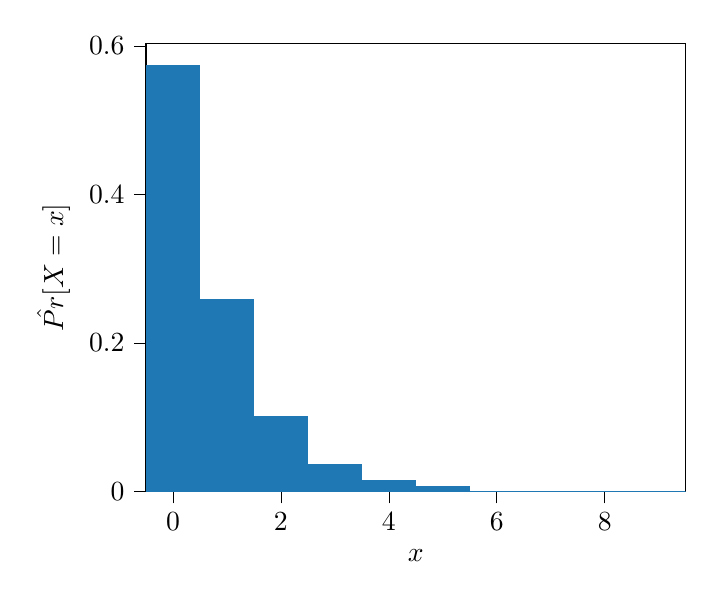
\begin{tikzpicture}

\definecolor{darkgray176}{RGB}{176,176,176}
\definecolor{steelblue31119180}{RGB}{31,119,180}

\begin{axis}[
tick align=outside,
tick pos=left,
x grid style={darkgray176},
xlabel={\(\displaystyle x\)},
xmin=-0.5, xmax=9.5,
xtick style={color=black},
y grid style={darkgray176},
ylabel={\(\displaystyle \hat{Pr}[X=x]\)},
ymin=0, ymax=0.603504672897201,
ytick style={color=black},
yticklabel style={/pgf/number format/fixed}
]
\draw[draw=none,fill=steelblue31119180] (axis cs:-0.5,0) rectangle (axis cs:0.5,0.574766355140192);
\draw[draw=none,fill=steelblue31119180] (axis cs:0.5,0) rectangle (axis cs:1.5,0.259012016021365);
\draw[draw=none,fill=steelblue31119180] (axis cs:1.5,0) rectangle (axis cs:2.5,0.102136181575435);
\draw[draw=none,fill=steelblue31119180] (axis cs:2.5,0) rectangle (axis cs:3.5,0.0367156208277708);
\draw[draw=none,fill=steelblue31119180] (axis cs:3.5,0) rectangle (axis cs:4.5,0.0153538050734314);
\draw[draw=none,fill=steelblue31119180] (axis cs:4.5,0) rectangle (axis cs:5.5,0.00801068090787727);
\draw[draw=none,fill=steelblue31119180] (axis cs:5.5,0) rectangle (axis cs:6.5,0.00133511348464621);
\draw[draw=none,fill=steelblue31119180] (axis cs:6.5,0) rectangle (axis cs:7.5,0.00133511348464621);
\draw[draw=none,fill=steelblue31119180] (axis cs:7.5,0) rectangle (axis cs:8.5,0.000667556742323105);
\draw[draw=none,fill=steelblue31119180] (axis cs:8.5,0) rectangle (axis cs:9.5,0.000667556742323105);
\end{axis}

\end{tikzpicture}

	$$\hat{Pr}_{128}[X=0] \approx 0.57$$
\end{frame}

\begin{frame}{Improving the Reliability of the Meteor Stegosystem}
	\centering
	% This file was created with tikzplotlib v0.10.1.
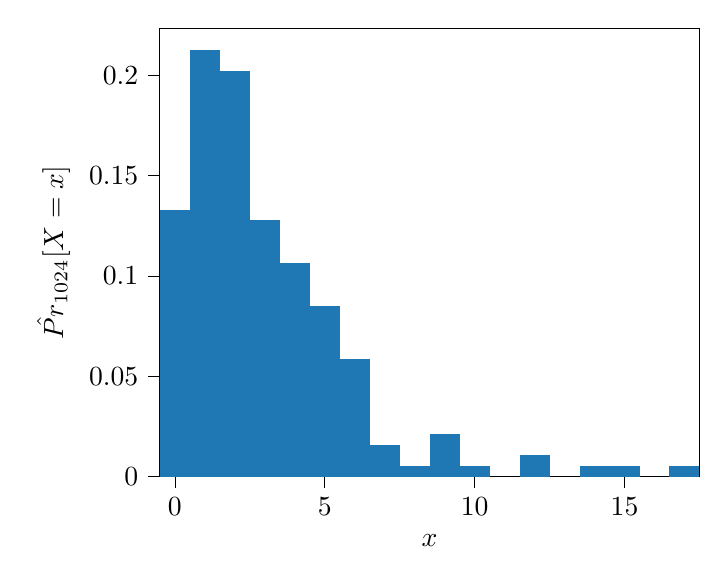
\begin{tikzpicture}

\definecolor{darkgray176}{RGB}{176,176,176}
\definecolor{steelblue31119180}{RGB}{31,119,180}

\begin{axis}[
tick align=outside,
tick pos=left,
x grid style={darkgray176},
xlabel={\(\displaystyle x\)},
xmin=-0.5, xmax=17.5,
xtick style={color=black},
y grid style={darkgray176},
ylabel={\(\displaystyle \hat{Pr}_{1024}[X=x]\)},
ymin=0, ymax=0.223404255319149,
ytick style={color=black},
yticklabel style={/pgf/number format/fixed}
]
\draw[draw=none,fill=steelblue31119180] (axis cs:-0.5,0) rectangle (axis cs:0.5,0.132978723404255);
\draw[draw=none,fill=steelblue31119180] (axis cs:0.5,0) rectangle (axis cs:1.5,0.212765957446808);
\draw[draw=none,fill=steelblue31119180] (axis cs:1.5,0) rectangle (axis cs:2.5,0.202127659574468);
\draw[draw=none,fill=steelblue31119180] (axis cs:2.5,0) rectangle (axis cs:3.5,0.127659574468086);
\draw[draw=none,fill=steelblue31119180] (axis cs:3.5,0) rectangle (axis cs:4.5,0.106382978723405);
\draw[draw=none,fill=steelblue31119180] (axis cs:4.5,0) rectangle (axis cs:5.5,0.085106382978724);
\draw[draw=none,fill=steelblue31119180] (axis cs:5.5,0) rectangle (axis cs:6.5,0.0585106382978727);
\draw[draw=none,fill=steelblue31119180] (axis cs:6.5,0) rectangle (axis cs:7.5,0.0159574468085107);
\draw[draw=none,fill=steelblue31119180] (axis cs:7.5,0) rectangle (axis cs:8.5,0.00531914893617025);
\draw[draw=none,fill=steelblue31119180] (axis cs:8.5,0) rectangle (axis cs:9.5,0.021276595744681);
\draw[draw=none,fill=steelblue31119180] (axis cs:9.5,0) rectangle (axis cs:10.5,0.00531914893617025);
\draw[draw=none,fill=steelblue31119180] (axis cs:10.5,0) rectangle (axis cs:11.5,0);
\draw[draw=none,fill=steelblue31119180] (axis cs:11.5,0) rectangle (axis cs:12.5,0.0106382978723405);
\draw[draw=none,fill=steelblue31119180] (axis cs:12.5,0) rectangle (axis cs:13.5,0);
\draw[draw=none,fill=steelblue31119180] (axis cs:13.5,0) rectangle (axis cs:14.5,0.00531914893617025);
\draw[draw=none,fill=steelblue31119180] (axis cs:14.5,0) rectangle (axis cs:15.5,0.00531914893617025);
\draw[draw=none,fill=steelblue31119180] (axis cs:15.5,0) rectangle (axis cs:16.5,0);
\draw[draw=none,fill=steelblue31119180] (axis cs:16.5,0) rectangle (axis cs:17.5,0.00531914893617025);
\end{axis}

\end{tikzpicture}

	$$\hat{Pr}_{1024}[X=0] \approx 0.13$$
\end{frame}

\begin{frame}{Improving the Reliability of the Meteor Stegosystem}
	\begin{itemize}[<+->]
		\item \textbf{Can we recover} from decoding failures? 
		\item Good news: \textbf{Yes}, we can!
		\item Bad news: \textbf{exponential computational overhead} (potentially).
	\end{itemize}
\end{frame}

\begin{frame}{Improving the Reliability of the Meteor Stegosystem}
	\begin{itemize}[<+->]
		\item A: \textbf{split hiddentext} into blocks of size $\gamma$, add \textbf{checksums} of size $\delta$.
		\item B: \textbf{verify checksums} while decoding stegotext $c$.
		\item If \textbf{verification fails}, a tokenization mismatch in word $c_w$ occurred.
		\item Generate \textbf{tokenization graph} $G=(V,E)$ of $c_w$.
		\item Find all paths in $G$ and \textbf{retry with a random path}.
		\item \textbf{Worst case}: $c_w$ has $2^{\left|V\right|-2} = 2^{|c_w|-1}$ paths in $G$.
		\item \textbf{Average case}: $|c_w| = 5$, up to 16 tokenizations (GPT tokenizer).
	\end{itemize}
\end{frame}

\section{Conclusion}

\begin{frame}{Conclusion}
    \begin{itemize}[<+->]
        \item \textbf{Generative models} can be used to build \textbf{secure stegosystems}.
        \item Ambiguous tokenization causes \textbf{computational overhead}.
        \item Meteor is \textbf{easily adaptable} to different models, e.g., DialoGPT.
        \item We can \textbf{improve security} by replacing cryptographic primitive.
        \item Improved \textbf{hardware support} and \textbf{model performance}.
    \end{itemize}
\end{frame}
	


\section*{Appendix}

\begin{frame}{Appendix: Improving the Reliability of the Meteor Stegosystem}
  \centering
  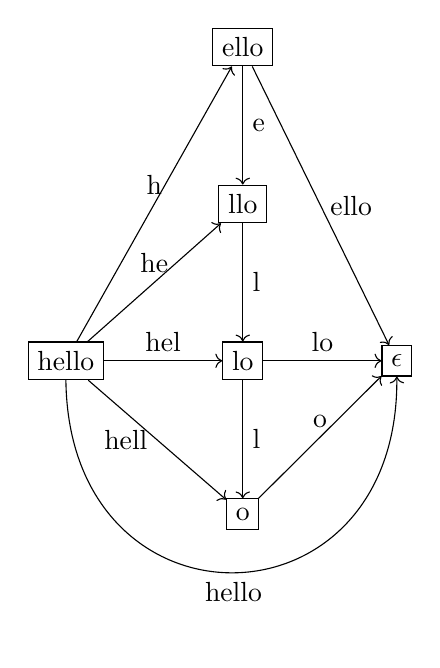
\begin{tikzpicture}
    \node[rectangle, draw=black] (hello) {hello};
    \node[rectangle, draw=black, right=15mm of hello] (lo) {lo};
    \node[rectangle, draw=black, above=15mm of lo] (llo) {llo};
    \node[rectangle, draw=black, above=15mm of llo] (ello) {ello};
    \node[rectangle, draw=black, below=15mm of lo] (o) {o};
    \node[rectangle, draw=black, right=15mm of lo] (bot) {$\epsilon$};
    
    \draw[->] (hello) to node[above] {h} (ello);
    \draw[->] (hello) to node[above] {he} (llo);
    \draw[->] (hello) to node[above] {hel} (lo);
    \draw[->] (hello) to node[left] {hell} (o);
    \draw[->, bend right=90,looseness=2] (hello) to node[below] {hello} (bot);

    \draw[->] (ello) to node[right] {e} (llo);
    %\draw[->, bend left=30] (ello) to node[right] {el} (lo);
    %\draw[->, bend left=30] (ello) to node[above] {ell} (o);
    \draw[->] (ello) to node[right] {ello} (bot);

    \draw[->] (llo) to node[right] {l} (lo);
    %\draw[->, bend right=30] (llo) to node[above] {ll} (o);
    %\draw[->] (llo)   to node[above] {llo} (bot);

    \draw[->] (lo)    to node[right] {l} (o);
    \draw[->] (lo)    to node[above] {lo} (bot);

    \draw[->] (o)     to node[above] {o} (bot);
  \end{tikzpicture}
\end{frame}

\begin{frame}{Appendix: Improving the Security of the Meteor Stegosystem}
	\begin{itemize}
		\item \textbf{SS-CHA security} by reduction to PRG.
		\item Meteor's implementation is \textbf{deterministic}.
		\item \textbf{Secure} against CHA with query complexity one.
		\item \textbf{Insecure} against CHA with higher query complexity.
		\item \textbf{Improve security with SES-CTR} to randomize outputs.
	\end{itemize}
\end{frame}

\begin{frame}{Appendix: Meteor One-Way (Example with GPT-2)}
	\centering
	\includegraphics[height=0.9\textheight]{twoway_no_split.png}
\end{frame}

\begin{frame}{Appendix: Meteor Conversation (Example with GPT-2)}
	\centering
	\includegraphics[height=0.9\textheight]{twoway_gpt.png}
\end{frame}

\begin{frame}{Appendix: Meteor Conversation (Example with DialoGPT)}
	\centering
	\includegraphics[height=0.9\textheight]{twoway_dialogpt.png}
\end{frame}

\end{document}